%!TEX root = ..\lections.tex
\section{Изолированные и неизолированные периодические траектории. Определение предельного цикла}%
\label{sec:7.1}

На предыдущих лекциях мы рассмотрели один из главных типов
траекторий динамических систем – состояния (положения) равновесия,
которым соответствуют состояния покоя реальных систем. Другой важный
класс траекторий образуют так называемые \textbf{предельные циклы} , которым
соответствуют периодические изменения во времени реальных систем.
Рассмотрим предельные циклы динамических систем, заданных на фазовой
плоскости

\begin{equation}
        \label{eq:7.1}
        \begin{cases}
                \dot x_1 = f_1(x_1,x_2), \\
                \dot x_2 = f_2(x_1,x_2). 
        \end{cases}
\end{equation}
Поскольку предельный цикл отображает периодические во времени процессы
реальных систем, то на фазовой плоскости он должен быть представлен
замкнутой фазовой траекторией. С замкнутыми фазовыми траекториями мы
уже встречались при изучении динамики нелинейного осциллятора, который,
если имеет на фазовой плоскости периодические траектории, то их всегда
континуум. Принципиальное отличие предельных циклов от периодических
траекторий консервативных систем состоит в том, что они обладают свойством
изолированности.\textbf{Замкнутая фазовая траектория называется
изолированной, если существует достаточно малая кольцеобразная
окрестность этой траектории, внутри которой нет других замкнутых
траекторий.} Поясним смысл этого свойства на примере двух следующих
систем
\begin{equation}
        \label{eq:7.2}
        \dot x_1 = -x_2,\quad \dot x_2 = x_1
\end{equation}
и
\begin{equation}
        \label{eq:7.3}
        \begin{cases}
                \dot x_1 = -x_2 + x_1(1-x_1^2 - x_2^2), \\
                \dot x_2 = x_1 +x_2(1-x_1^2 - x_2 ).      
        \end{cases}
\end{equation}
Система \eqref{eq:7.2} -- гармонический осциллятор, фазовый портрет которого представлен на рис.\ref{fig:7.1}a. Система \eqref{eq:7.2} имеет континуум замкнутых траекторий вида: $x_1^2+x_2^2 = C,$ 
где $C= \const>0$. Ясно, что в этом случае ни одна из замкнутых траекторий не является изолированной.
\begin{figure}[h]
        \centering
        \begin{minipage}{0.49\linewidth}
                \centering
                %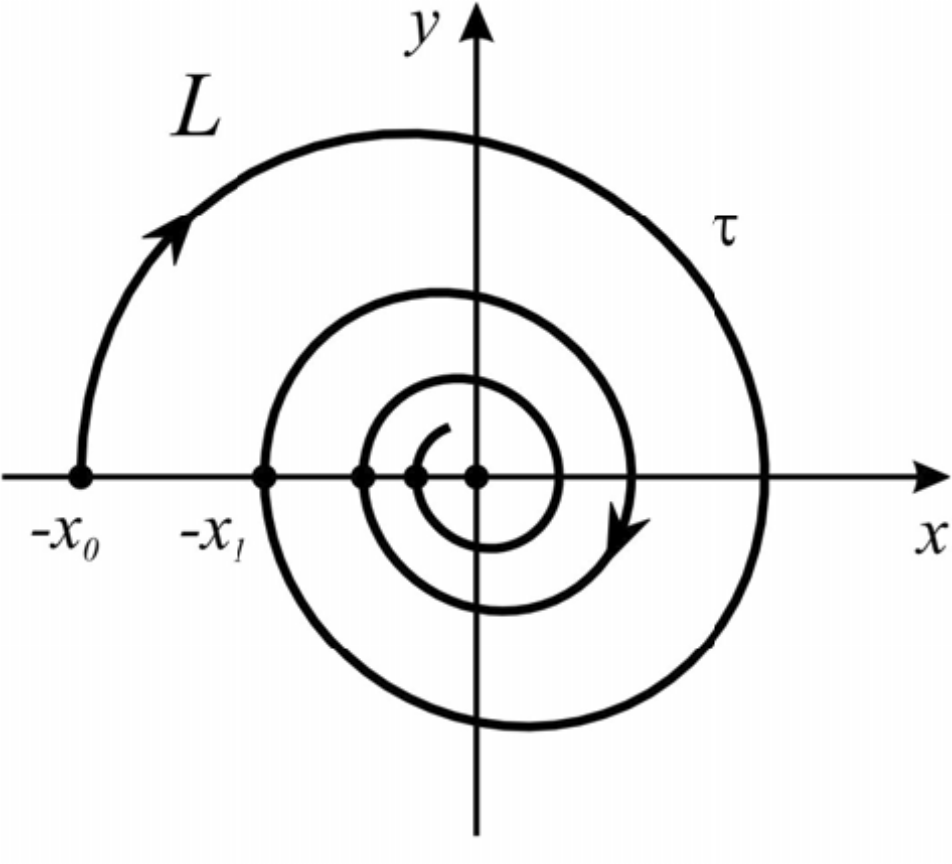
\includegraphics[width=\linewidth]{fig/lect7/1a}
                (a)
        \end{minipage}
        \begin{minipage}{0.49\linewidth}
                \centering
                %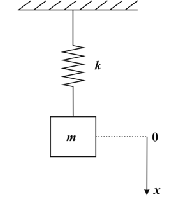
\includegraphics[width=\linewidth]{fig/lect7/1b}
                (b)
        \end{minipage}
        \caption{Фазовые портреты системы \eqref{eq:7.2} (а) и системы \eqref{eq:7.3} (b).}
        \label{fig:7.1}
\end{figure}
Построим теперь фазовый портрет системы \eqref{eq:7.3}. Для этого перейдем в \eqref{eq:7.3} к полярным координатам
\begin{equation}
        \label{eq:7.4}
        x_1 = \rho \cos \phi, \quad x_2 = \rho \sin \phi.
\end{equation}
Подставляя \eqref{eq:7.4} в систему \eqref{eq:7.3}, получим
\begin{equation}
        \label{eq:7.5}
        \begin{cases}
                \dot \rho \cos \phi - \rho \sin \phi \cdot \phi = - \rho \sin \phi + \rho(1-\rho^2)\cos \phi,\\
                \dot \phi \sin \phi + \rho \cos \phi \cdot \phi = \rho \cos \phi + \rho(1-\rho^2)\sin \phi.
        \end{cases}
\end{equation}
Разрешая \eqref{eq:7.5} относительно производных, находим уравнения для $\rho$ и $\phi$
 \begin{equation}
        \label{eq:7.6}
        \dot \rho = \rho(1-\rho),\quad \dot \phi =1.
\end{equation}
Первое уравнение в системе \eqref{eq:7.6} имеет два состояния равновесия --
неустойчивое в точке  $\rho=0$ и устойчивое в точке $\rho=1$, а угловая переменная
изменяется в соответствии с уравнением $\phi = t + \phi_0$ , где $\phi_0= \const$. Принимая во
внимание эти свойства, устанавливаем фазовый портрет системы \eqref{eq:7.3},
представлений на рис. \ref{fig:7.1}b. На фазовой плоскости существует единственная
замкнутая изолированная фазовая траектория – предельный цикл $L_0$. Пусть при
$t=t_0$ переменная $\phi(t_0)=0$. Тогда из уравнения $\phi(t_0)= t_0+ \phi_0$ находим, что $\phi_0=-t_0$ .
Отсюда и \eqref{eq:7.4} получаем, что предельный цикл
$L_0$  задается следующим
образом $L_0 = \qty{x_1=\cos(t-t_0),~ x_2 = \sin(t-t_0)}$ (заметим, что в неявном виде цикл
$L_0$ задается уравнением $x_1^2+x_2^2=1$). Цикл
$L_0$ притягивает все, кроме состояния
равновесия $x_1=x_2=0$, траектории системы \eqref{eq:7.3}. Следовательно, в отличии от
периодических движений консервативных систем, амплитуда которых
определяется начальными условиями, периодические движения, отвечающие
предельным циклам, имеют характеристики (амплитуду, период) в
определенных пределах независящие от начальных условий (в случае системы
\eqref{eq:7.3} характеристики цикла $L_0$ вообще не зависят от начальных условий) и, как
будет показано позднее, полностью определяются параметрами динамической системы.

Таким образом, \textbf{предельным циклом называется замкнутая изолированная фазовая траектория.} 
Предельному циклу соответствует периодическое решение системы \eqref{eq:7.1}, т.е.
\begin{equation}
        \label{eq:7.7}
        L_0 = \qty{ x_1=x_1^*(t), ~ x_2=x_2^*(t)},
\end{equation}
где $x_i^* (t+T_0)= x_i^*(t),~i=1,2,~ T_0(T_0>0)$--минимальный период. Заметим, что форма 
периодических колебаний, отвечающих предельным циклам, может меняться в самых широких
пределах -- от синусоидальной (например, как в системе \eqref{eq:7.3}) до кноидальной.

\section{Орбитальная устойчивость. Устойчивые и неустойчивые предельные циклы.}%
\label{sec:7.2}

Предположим, что система \eqref{eq:7.1} имеет предельный цикл $L_0$ и существует такая кольцеобразная
окрестность цикла, что все траектории, начинающиеся в этой окрестности, асимптотически приближаются к предельному циклу $L_0$ (см. рис.\ref{fig:7.2}a). Следовательно, цикл $L_0$ обладает признаками устойчивого поведения. Однако, из-за неизохронности траекторий в окрестности $L_0$ определение устойчивости по Ляпунову в этом случае не выполняется и является слишком жестким.
\begin{figure}[h]
        \centering
        \begin{minipage}{0.49\linewidth}
               \centering
               \includegraphics[width=0.6\linewidth]{example-image-a} 

               (a)
        \end{minipage}
        \begin{minipage}{0.49\linewidth}
               \centering
               \includegraphics[width=0.6\linewidth]{example-image-a} 

               (b)
        \end{minipage}
        \caption{Предельные циклы: устойчивый (a); неустойчивый (b)}
        \label{fig:7.2}
\end{figure}

\subsection{Определение орбитальной устойчивости}%
\label{sub:7.2.1}

Для преодоления этого противоречия в случае периодических траекторий вводят понятие так называемой
орбитальной устойчивости, обладающей менее жесткими ограничениями. Сформулируем это определение для системы произвольной размерности
(система \eqref{eq:3.1}, лекция \ref{lect3}). Пусть $L=\qty{\vec x = \vec x^*(t)}$, где
$\vec x^*(t+T_0)=\vec x^*(t)$, -- периодическая траектория системы \eqref{eq:3.1}.

\definition{\label{def:7.1}
        Периодическая траектория $L$ называется орбитально устойчивой при $ t\to + \infty$, если для любого $\epsilon > 0 $ существует число $\delta=\delta(\epsilon,t_0)$ такое, что любая полутраектория $\vec x(t),~t_0\leq t < + \infty$, для которой 
        \begin{equation}
                \label{eq:}
                \norm{ \vec x(t) - \vec x^* (t) } < \delta,
        \end{equation}
в дальнейшем целиком содержится в $\epsilon$-окрестности траектории $L$, т.е.
\begin{equation}
        \label{eq:}
        \rho\qty( \vec x(t),L) < \epsilon \text{ при }  t\geq t_0,
\end{equation}
где $\rho\qty( \vec x(t),L)$ -- минимальное евклидово расстояние от $\vec x(t)$ до траектории $L$ :
\begin{equation}
        \label{eq:}
        \rho\qty( \vec x (t), L) = \underset{L}{\mathrm{inf}} \norm{ \vec x(t)-L}.
\end{equation}

Кроме того, если для всех траекторий, достаточно близких к $L$, расстояние $\rho\qty(\vec x(t),L)\to 0 $} при $t \to + \infty$, то траектория $L$ называется \textbf{орбитально асимптотически устойчивой.} Если же в сколь угодно малой окрестности существует хотя бы одна фазовая траектория, покидающая окрестность $L$ при $t \to + \infty$, то траектория называется неустойчивой.
        
Очевидно, что предельный цикл $L_0$ системы \eqref{eq:7.3}, представленный на рис.\ref{fig:7.1}a, является орбитально асимптотически устойчивым (далее для краткости устойчивым), а на рис.\ref{fig:7.2}b -- неустойчивым.

\subsection{Характеристики предельных циклов}%
\label{sub:7.2.2}

Пусть $L_0$ -- предельный цикл системы \eqref{eq:7.1}. Зафиксируем на $L_0$ произвольную точку и проведем
в этой точке касательную к $L_0$, а к ней -- ортогональную прямую $N$ (см. рис.\ref{fig:7.3}). Введем на $N$ координату так, чтобы начало координат было в точке пересечения $N$ и $L_0$. Рассмотрим поведение траекторий системы \eqref{eq:7.1} в малой
кольцеобразной окрестности предельного цикла $L_0$. Поскольку время
движения вдоль предельного цикла $L_0$ конечно, то в силу теоремы о
непрерывной зависимости решений дифференциальных уравнений от
начальных условий любая траектория системы \eqref{eq:7.1} из малой окрестности  $L_0$,
<<стартующая>> с прямой $N$ из точки $\xi$ , через конечное время вернется на
прямую $N$ в некоторой точке с координатой $\xi$ . Другими словами, прямая $N$
является локальной секущей Пуанкаре, на которой траектории системы \eqref{eq:7.1}
порождают точечное отображение Пуанкаре
\begin{equation}
        \label{eq:7.8}
        \bar \xi = g(\xi).
\end{equation}
\begin{figure}[h]
        \centering
        \includegraphics[width=0.6\linewidth]{example-image-a}
        \caption{Генерация отображения Пуанкаре в окрестности предельного цикла.}
        \label{fig:7.3}
\end{figure}
Рассмотрим качественный вид функции последования $g( \xi)$ в случае устойчивого и неустойчивого предельных циклов. Так как из малой окрестности устойчивого предельного цикла все траектории системы
\eqref{eq:7.1} асимптотически приближаются к циклу, то траектории соответствующего точечного отображения асимптотически стремятся к неподвижной точке $\xi = 0$ отображения \eqref{eq:7.8}. Качественный вид отображения \eqref{eq:7.8} в этом случае представлен на рис.\ref{fig:7.4}a. Рассуждая совершенно аналогично, устанавливаем качественный вид отображения \eqref{eq:7.8} для неустойчивого предельного цикла (см. рис.\ref{fig:7.4}b).
\begin{figure}[h]
        \centering
        \begin{minipage}{0.49\linewidth}
                \centering
               \includegraphics[width=0.6\linewidth]{example-image-a} 

               (a)
        \end{minipage}
        \begin{minipage}{0.49\linewidth}
                \centering
               \includegraphics[width=0.6\linewidth]{example-image-a} 

               (b)
        \end{minipage}
        \caption{Качественный вид отображения Пуанкаре в окрестности устойчивого (a) и неустойчивого (b) предельных циклов.}
        \label{fig:7.4}
\end{figure}
Следовательно, между устойчивостью предельных циклов и
неподвижных точек соответствующих отображений Пуанкаре существует
взаимно-однозначное соответствие. Это позволяет ввести характеристику
предельного цикла -- мультипликатор предельного цикла, как мультипликатор
соответствующей неподвижной точки отображения \eqref{eq:7.16}, т.е. как величину
\begin{equation}
        \label{eq:7.9}
        s = \dv{g}{\xi} \eval_{\xi=0} = g'(0),
\end{equation}
которая для предельных циклов на плоскости всегда является положительной.
Мультипликатор устойчивого предельного цикла удовлетворяет неравенству
$s<1$, а неустойчивого -- $s>1$. Заметим, что, если уравнение предельного цикла
известно, его мультипликатор может быть найден следующим образом
\begin{equation}
        \label{eq:7.10}
        s= \exp{ \int\limits_{0}^{T_0} 
        \qty[\pdv{f_1}{x_1}\eval_{x^*(t)} +
        \pdv{f_2}{x_2}\eval_{x^*(t)}]\dd{t}}, 
\end{equation}

Другой характеристикой предельных циклов является так называемый \textbf{характеристический показатель}. Его можно ввести следующим образом. Линеаризуем систему \eqref{eq:7.1} на цикле $L_0$, полагая $x_i = x^*_i(t) + \eta_i, ~ i =1,2$
и разлагая правые части системы  \eqref{eq:7.1} в ряды по степеням $\eta_i$. Тогда в линейном приближении получим
\begin{equation}
        \label{eq:7.11}
        \dot \eta_i = \sum\limits_{j=1}^{2} a_{ij}(t) \eta_j(t), ~ i = 1,2,
\end{equation}
где 
\begin{equation}
        \label{eq:}
        a_{ij}(t) = \pdv{f_i}{x_j} \eval_{x^*(t)}, \quad a_{ij}(t+T_0)= a_{ij}(t).
\end{equation}
Система \eqref{eq:7.11} является линейной системой с периодическими коэффициентами. Общее решение системы \eqref{eq:7.11} определяется теорией Флоке и имеет вид
\begin{equation}
        \label{eq:}
        \eta_i(t) = \sum\limits_{j=1}^{2} C_j \Phi_{ij}(t) e^{\lambda_j t}, ~ i =1,2,
\end{equation}
где $C_j = \const,$ а $\Phi_{ij}$ -- периодические функции периода $T_0$, а $\lambda_j$ - постоянные называемые характеристическими показателями. Согласно теореме Андронова-Понтрягина 
для автономных динамических систем один из характеристических показателей всегда равен нулю, а второй равен
\begin{equation}
        \label{eq:7.13}
        \lambda = \frac{1}{T_0}\ln s
\end{equation}

\section{Вращательные и колебательные предельные циклы}%
\label{sec:7.3}

Мы рассмотрели предельные циклы на фазовой плоскости. Однако
существуют такие реальные системы, для адекватного описания поведения
которых необходимо введение цилиндрического фазового пространства. Это
системы, у которых одна из переменных является угловой. Типичным
примером таких систем является обычный физический маятник. В
динамических системах с цилиндрическим фазовым пространством могут
существовать предельные циклы двух видов – вращательные и колебательные.
Первые из них охватывают фазовый цилиндр
$G = S^1 \times \R^1$ (см. рис.\ref{fig:7.5}a)
 и угловая
переменная вдоль цикла непрерывно нарастает. Колебательные циклы не
охватывают фазовый цилиндр $G$ (см. рис.\ref{fig:7.5}a), а лежат на поверхности цилиндра и
угловая координата колеблется около некоторого среднего значения.
\begin{figure}[h]
        \begin{minipage}{0.49\linewidth}
            \centering
            \includegraphics[width=0.6\linewidth]{example-image-a}
        \end{minipage}
        \begin{minipage}{0.49\linewidth}
            \centering
            \includegraphics[width=0.6\linewidth]{example-image-a}
        \end{minipage}
        \caption{Предельные циклы в цилиндрическом фазовом пространстве:
        вращательный (a);
        колебательный (b).}
        \label{fig:7.5}
\end{figure}


\section{Критерий Бендиксона-Дюлака}%
\label{sec:7.4}

Ясно, что для конкретных двумерных динамических систем задача о
существовании или, наоборот, отсутствии предельных циклов является
центральной. При этом доказательство отсутствия у системы предельных
циклов не менее важно с практической точки зрения, чем доказательство
противоположного утверждения. Действительно, если удалось установить
отсутствие предельных циклов, то динамика системы полностью понятна – при
любых начальных условиях система приходит в одно из равновесных
состояний. Одним из эффективных критериев выделения систем без замкнутых
траекторий является критерий Бендиксона-Дюлака: \textbf{если существует такая
        непрерывная с непрерывными производными функция $B(x_1,x_2)$, что в
некоторой односвязной области на фазовой плоскости выражение}
\begin{equation}
        \label{eq:}
        \pdv{x_1} (Bf_1) + \pdv{x_2} (B f_2)
\end{equation}
\textbf{знакопостоянно, то в этой области не существует замкнутых контуров,
целиком составленных из фазовых траекторий системы \eqref{eq:7.1}}.

Заметим, что критерий Бендиксона-Дюлака дает достаточные условия
отсутствия замкнутых фазовых траекторий. Этот критерий также применим и
для систем с цилиндрическим фазовым пространством. В этом случае
выполнение критерия Бендиксона-Дюлака в некоторой области, заключённой
между двумя замкнутыми кривыми, охватывающими фазовый цилиндр,
означает, что в этой области не существует колебательных предельных циклов,
и не может быть более одного вращательного предельного цикла.
